\section{Fluxo de desenvolvimento}\label{sec:figs}

Para desenvolver em um repositório precisamos usar uma branch, ou ramificação no português. Por padrão, todo repositório gerado pelo template possui uma branch chamada main. Essa branch possui uma configuração automática onde toda vez que é feita uma nova versão dela é gerada uma nova release no repositório. A image~\ref{fig:image05} mostra a ultima versao do template na plataforma do Github.

\begin{figure}[ht]
	\centering
	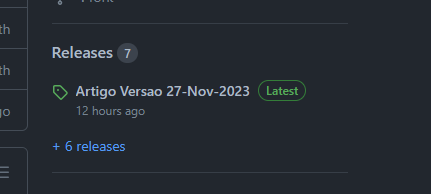
\includegraphics[width=.5\textwidth]{./images/image06.png}
	\caption{Ultima release}
	\label{fig:image06}
\end{figure}


Ao clicar na release, vai aparecer as informações da data da release junto com o arquivo em pdf (imagem~\ref{fig:image07}). isso permitirá que as pessoas com acesso ao repositório peguem a ultima versão do pdf sem a necessidade de abrir o latex.

\begin{figure}[ht]
	\centering
	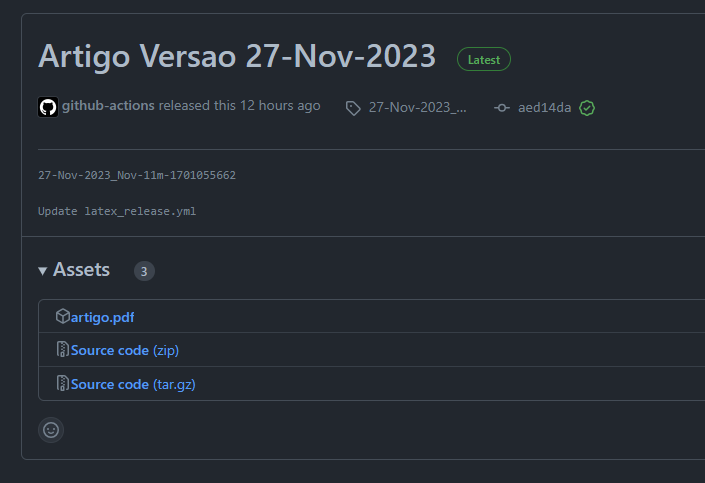
\includegraphics[width=.5\textwidth]{./images/image07.png}
	\caption{Detalhes da ultima release}
	\label{fig:image07}
\end{figure}

Para orientadores e outros envolvidos que não possuem o interesse ou a permissão para alterar o texto é uma funcionalidade bastante útil, pois evita de precisar gerar um novo pdf a cada acesso e mantém a confiabilidade da versão do tcc.
É possível ver as releases anteriores do tcc também. basta acessar a aba releases (imagem~\ref{fig:image08}), na tela da ultima release.


\begin{figure}[ht]
	\centering
	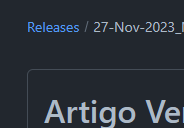
\includegraphics[width=.5\textwidth]{./images/image08.png}
	\caption{Aba releases}
	\label{fig:image08}
\end{figure}


\begin{figure}[ht]
	\centering
	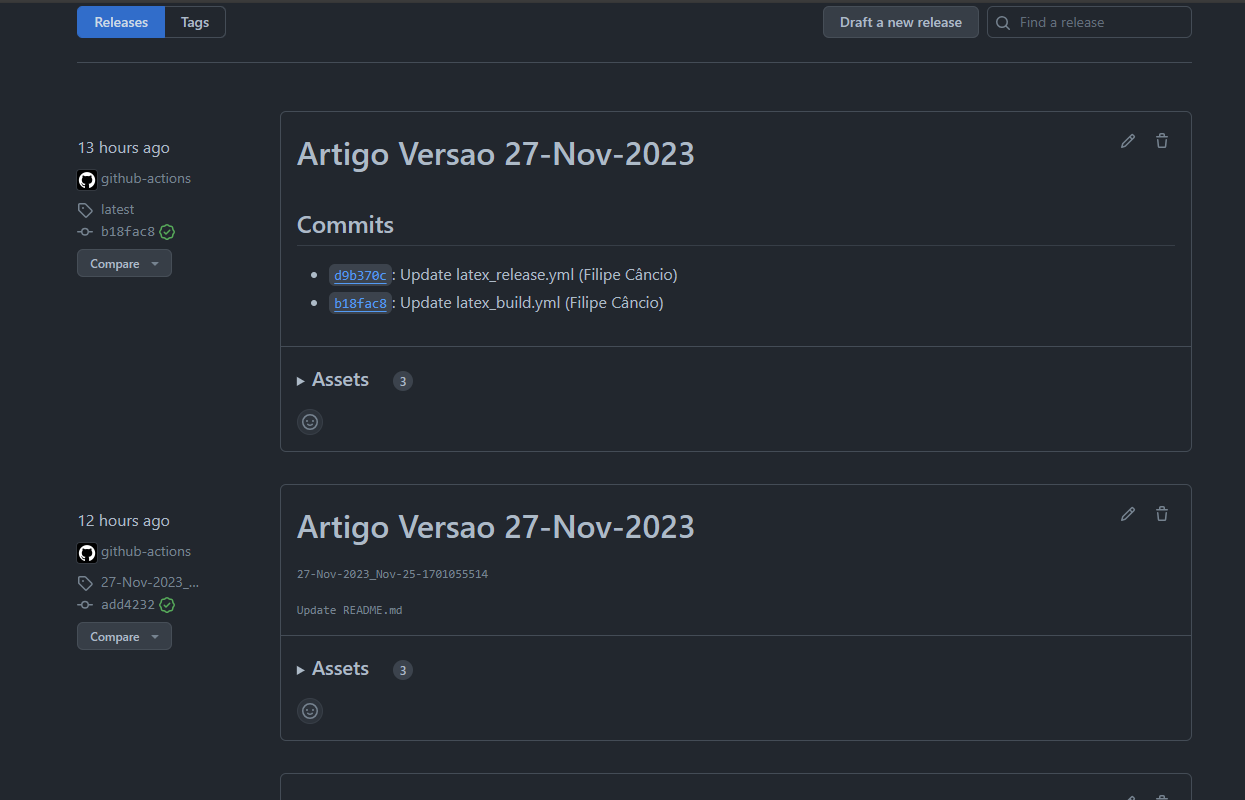
\includegraphics[width=.5\textwidth]{./images/image09.png}
	\caption{Lista de releases}
	\label{fig:image09}
\end{figure}

A utilização dessa funcionalidade permite ao autor a simples necessidade de subir o projeto para o repositório para cada versãoo ou se preferir alterar arquivos na própria plataforma.